\chapter{PENGUJIAN DAN EVALUASI}
\par Bab ini membahas pengujian dan evaluasi terhadap perangkat lunak yang telah diimplementasikan dengan menggunakan metode \textit{blackbox}.

\section{Lingkungan Pengujian}
\par Lingkungan yang digunakan untuk menguji tugas akhir ini memiliki spesifikasi perangkat keras dan lunak yang ditunjukkan pada Tabel \ref{t:spec-server}, \ref{t:spec-android}, \ref{t:spec-android-2}, \ref{t:spec-android-3} dan \ref{t:spec-ios}. Implementasi aplikasi android yang digunakan untuk pengujian dapat dilihat pada \nameref{lampiran:implementasi-android}.
\begin{longtable}{|p{3cm}|p{6cm}|}
	\caption{Spesifikasi Server} \label{t:spec-server} \\ \hline
    \rowcolor{lightgray} Komponen & Spesifikasi \\ \hline
    CPU & Intel(R) Xeon(R) CPU E5-2690 v4 \\ \hline
    CPU Core & 4 \\ \hline
    Memory & 8 GB \\ \hline
    Sistem Operasi & Ubuntu 18.04 \\ \hline
\end{longtable}
\begin{longtable}{|p{3cm}|p{6cm}|}
	\caption{Spesifikasi Perangkat Android 1} \label{t:spec-android} \\ \hline
	\rowcolor{lightgray} Komponen & Spesifikasi \\ \hline
    CPU & Snapdragon 636 \\ \hline
    Memory & 3 GB \\ \hline
    Sistem Operasi & Android 9 (Pie) \\ \hline
    Aplikasi & Push Notification Dev versi 1.0 \\ \hline
\end{longtable}
\pagebreak
\begin{longtable}{|p{3cm}|p{6cm}|}
\caption{Spesifikasi Perangkat Android 2} \label{t:spec-android-2} \\ \hline
\rowcolor{lightgray} Komponen & Spesifikasi \\ \hline
CPU & Snapdragon 625 \\ \hline
Memory & 4 GB \\ \hline
Sistem Operasi & Android 7 (Nougat) \\ \hline
Aplikasi & Push Notification Dev versi 1.0 \\ \hline
\end{longtable}
\begin{longtable}{|p{3cm}|p{6cm}|}
\caption{Spesifikasi Perangkat Android 3} \label{t:spec-android-3} \\ \hline
\rowcolor{lightgray} Komponen & Spesifikasi \\ \hline
CPU & Snapdragon 616 \\ \hline
Memory & 3 GB \\ \hline
Sistem Operasi & - \\ \hline
Aplikasi & Push Notification Dev versi 1.0 \\ \hline
\end{longtable}
\begin{longtable}{|p{3cm}|p{6cm}|}
	\caption{Spesifikasi Perangkat iOS} \label{t:spec-ios} \\ \hline
	\rowcolor{lightgray} Komponen & Spesifikasi \\ \hline
    CPU & Apple A10 Fusion \\ \hline
    Memory & 3 GB \\ \hline
    Sistem Operasi & iOS 12 \\ \hline
    Aplikasi & MyITS Wali versi 1.0.2 \\ \hline
\end{longtable}

\section{Pengujian Fungsional}
\par Pengujian fungsional dilakukan untuk mengetahui apakah sistem yang dibangun sudah memiliki kebutuhan fungsional yang diperlukan.

\subsection{Pengujian Pembuatan Packet}
\par Pengujian Pembuatan Packet dilakukan untuk mengetahui apakah Scheduler berhasil membuatkan data \textit{packet} dari \textit{batch} dengan tepat. Hasil uji dapat dilihat pada Tabel \ref{t:uji_pembuatan_packet}.
\begin{longtable}{|>{\columncolor{lightgray}}p{3cm}|p{6.5cm}|}
	\caption{Hasil Uji Pembuatan \textit{Packet}} \label{t:uji_pembuatan_packet} \\ \hline
	Kode & FT-01 \\ \hline
	Nama & Pengujian Pembuatan Packet \\ \hline
	Tujuan & Menguji apakah sistem mampu membuatkan data \textit{packet} dari data \textit{batch} \\ \hline
	Kondisi Awal & Scheduler aktif \\ \hline
	Langkah Pengujian &  
	\begin{enumerate}
		\item Pengguna menambahkan data \textit{batch} baru lewat halaman kirim notifikasi di modul manajemen.
		\item Setelah 30 detik, data \textit{packet} akan disimpan di sistem basis data.
	\end{enumerate} \\ \hline
	Hasil yang diharapkan & Data \textit{packet} tersimpan di sistem basis data \\ \hline
	Hasil yang diperoleh & Data \textit{packet} tersimpan di sistem basis data \\ \hline
	Hasil pengujian & Berhasil \\ \hline
\end{longtable}

\subsection{Pengujian Menambahkan Packet ke Antrian}
\par Pengujian menambahkan \textit{packet} dilakukan untuk mengetahui apakah Scheduler berhasil menambahkan \textit{packet} ke antrian dengan tepat. Hasil uji dapat dilihat pada Tabel \ref{t:uji_pembuatan_antrian}.
\begin{longtable}{|>{\columncolor{lightgray}}p{3cm}|p{6.5cm}|}
	\caption{Hasil Uji Menambahkan \textit{Packet} ke Antrian} \label{t:uji_pembuatan_antrian} \\ \hline
	Kode & FT-02 \\ \hline
	Nama & Pengujian Pembuatan Antrian \\ \hline
	Tujuan & Menguji apakah sistem mampu membuatkan data antrian dari data \textit{packet} \\ \hline
	Kondisi Awal & Scheduler aktif \\ \hline
	Langkah Pengujian &  
	\begin{enumerate}
		\item Pengguna menambahkan data \textit{batch} baru lewat halaman kirim notifikasi di modul manajemen.
		\item 30 detik setelah waktu pengiriman \textit{batch}, data \textit{packet} untuk \textit{batch} akan tersimpan di sistem antrian pesan.
	\end{enumerate} \\ \hline
	Hasil yang diharapkan & Data \textit{packet} tersimpan di sistem antrian pesan. \\ \hline
	Hasil yang diperoleh & Data \textit{packet} tersimpan di sistem antrian pesan. \\ \hline
	Hasil pengujian & Berhasil \\ \hline
\end{longtable}

\subsection{Pengujian Pengiriman Packet ke APNs}
\par Pengujian pengiriman \textit{packet} ke APNs dilakukan untuk mengetahui apakah Sender APN berhasil mengirimkan \textit{packet} ke layanan APNs dengan tepat. Hasil uji dan notifikasi dapat dilihat pada Tabel \ref{t:uji_pengiriman_packet_apn} dan Gambar \ref{f:ss_ios}.
\begin{longtable}{|>{\columncolor{lightgray}}p{3cm}|p{6.5cm}|}
	\caption{Hasil Uji Pengiriman \textit{Packet} ke APNs} \label{t:uji_pengiriman_packet_apn} \\ \hline
	Kode & FT-03 \\ \hline
	Nama & Pengujian Pembuatan Packet \\ \hline
	Tujuan & Menguji apakah sistem mampu mengirim \textit{packet} lewat layanan APNs \\ \hline
	Kondisi Awal & Scheduler dan Sender APN aktif \\ \hline
	Langkah Pengujian &  
	\begin{enumerate}
		\item Pengguna menambahkan data \textit{batch} baru untuk perangkat iOS lewat halaman kirim notifikasi di modul Manajemen.
		\item 1 menit setelah waktu pengiriman \textit{batch}, notifikasi akan diterima oleh perangkat iOS.
	\end{enumerate} \\ \hline
	Hasil yang diharapkan & Notifikasi diterima oleh perangkat iOS \\ \hline
	Hasil yang diperoleh & Notifikasi diterima oleh perangkat iOS \\ \hline
	Hasil pengujian & Berhasil \\ \hline
\end{longtable}
\begin{figure}[H]
	\centering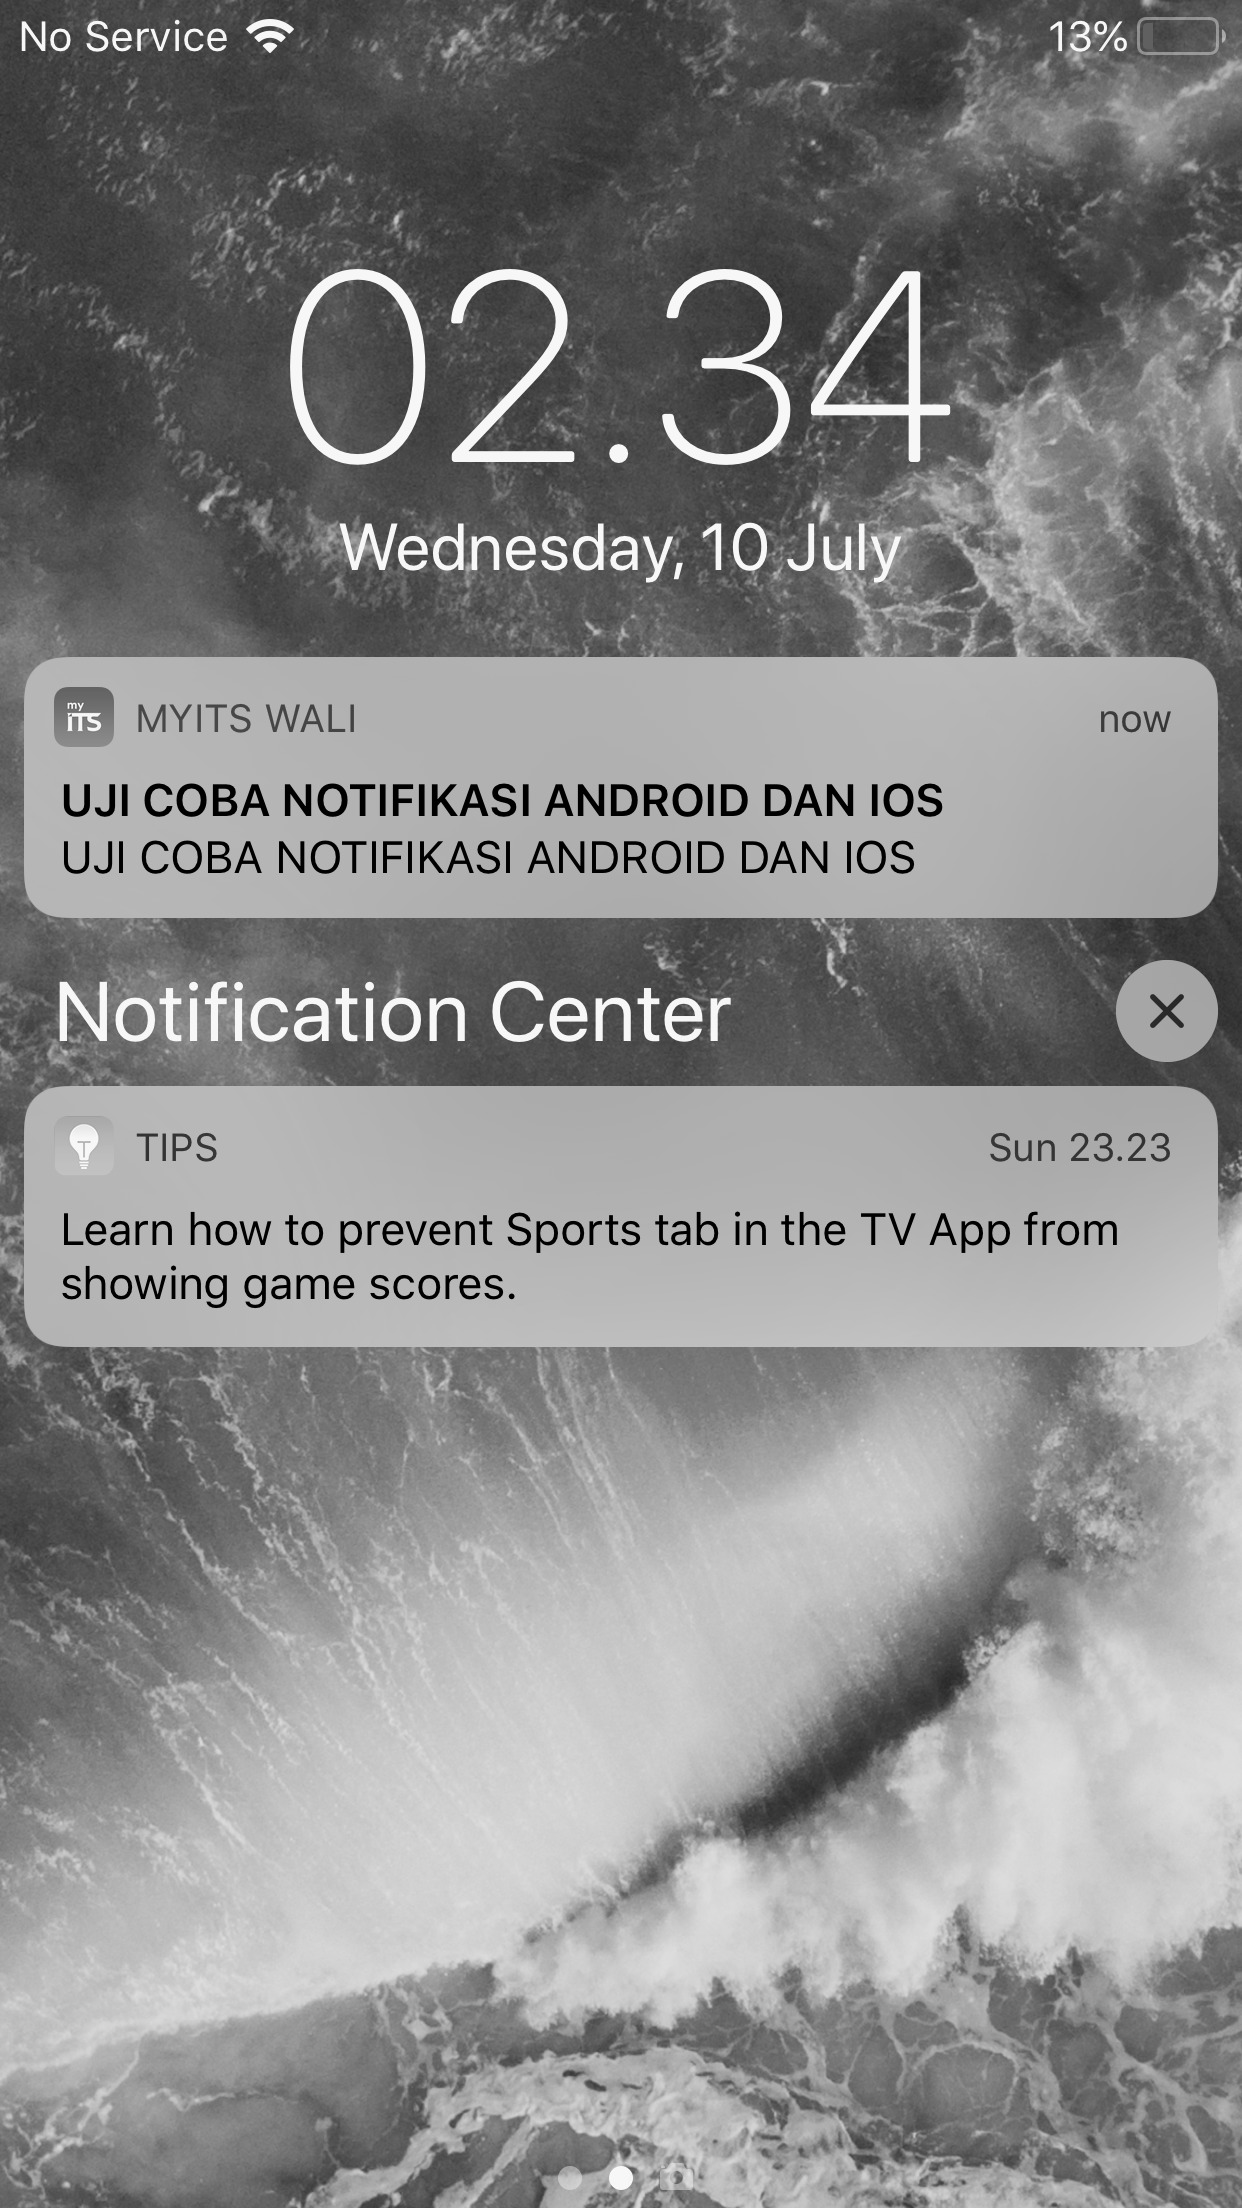
\includegraphics[width=0.4\textwidth]{bab5/img/notifikasi-ios.jpg}
	\caption{Hasil Notifikasi di Perangkat iOS} \label{f:ss_ios}
\end{figure}

\subsection{Pengujian Pengiriman Packet ke FCM}
\par Pengujian pengiriman \textit{packet} ke FCM dilakukan untuk mengetahui apakah Sender FCM berhasil mengirimkan \textit{packet} ke layanan FCM dengan tepat. Hasil uji dan notifikasi dapat dilihat pada Tabel \ref{t:uji_pengiriman_packet_fcm} dan Gambar \ref{img:notifikasi-android}.
\begin{longtable}{|>{\columncolor{lightgray}}p{3cm}|p{6.5cm}|}
	\caption{Hasil Uji Pengiriman \textit{Packet} ke FCM} \label{t:uji_pengiriman_packet_fcm} \\ \hline
	Kode & FT-04 \\ \hline
	Nama & Pengujian Pengiriman Packet ke FCM \\ \hline
	Tujuan & Menguji apakah sistem mampu mengirim \textit{packet} lewat layanan FCM \\ \hline
	Kondisi Awal & Scheduler dan Sender FCM aktif \\ \hline
	Langkah Pengujian &  
	\begin{enumerate}
		\item Pengguna menambahkan data \textit{batch} baru untuk perangkat Android lewat halaman kirim notifikasi di modul Manajemen.
		\item 1 menit setelah waktu pengiriman \textit{batch}, notifikasi akan diterima oleh perangkat Android.
	\end{enumerate} \\ \hline
	Hasil yang diharapkan & Notifikasi diterima oleh perangkat Android \\ \hline
	Hasil yang diperoleh & Notifikasi diterima oleh perangkat Android \\ \hline
	Hasil pengujian & Berhasil \\ \hline
\end{longtable}
\begin{figure}[H]
	\centering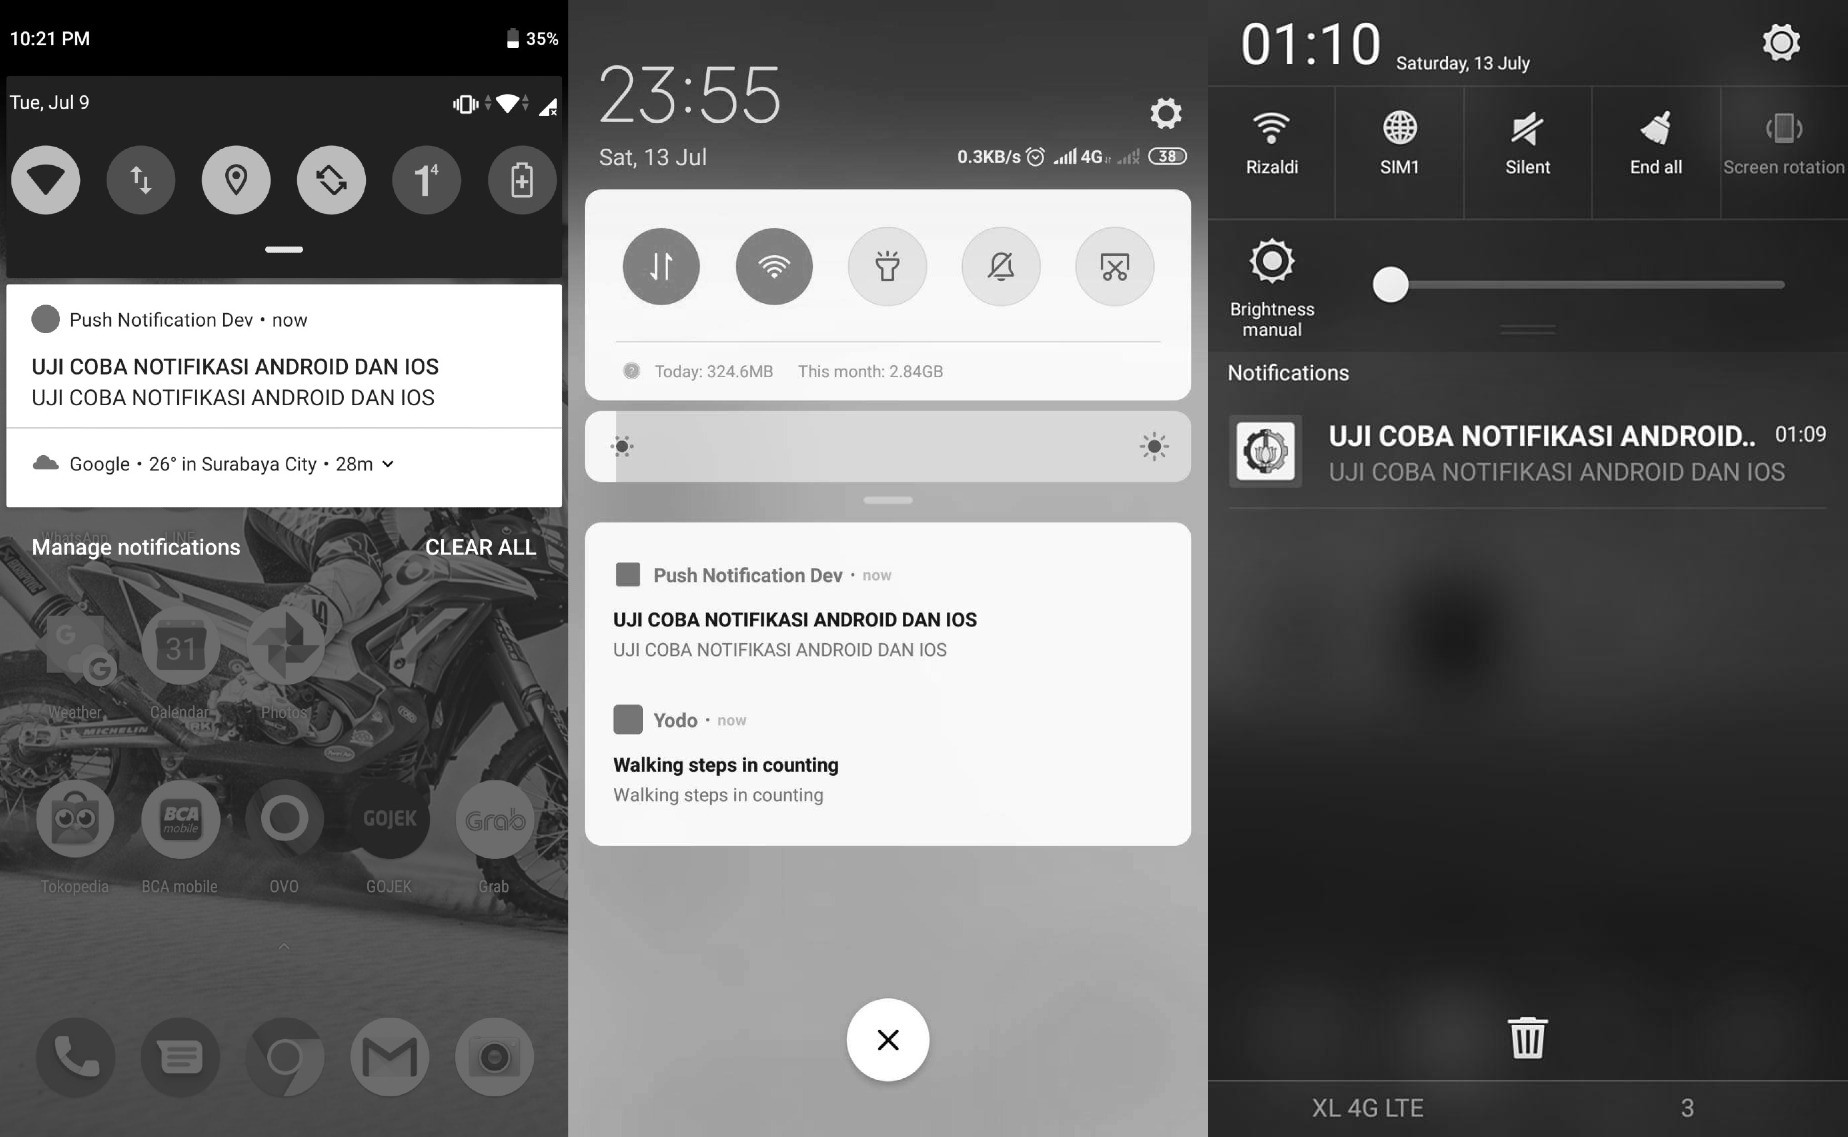
\includegraphics[width=1\textwidth]{bab5/img/notifikasi-android.jpg}
	\caption{Hasil Notifikasi di Perangkat Android 1, 2, dan 3} \label{img:notifikasi-android}
\end{figure}

\subsection{Pengujian Menampilkan Penggunaan Sumber Daya}
\par Pengujian menampilkan penggunaan sumber daya dilakukan untuk mengetahui apakah Scheduler, Sender APN, dan Sender FCM berhasil menampilkan penggunaan sumber daya dengan tepat. Hasil uji dapat dilihat pada Tabel \ref{t:uji_menampilkan_penggunaan_sumber_daya}.
\begin{longtable}{|>{\columncolor{lightgray}}p{3cm}|p{6.5cm}|}
	\caption{Hasil Uji Menampilkan Penggunaan Sumber Daya} \label{t:uji_menampilkan_penggunaan_sumber_daya} \\ \hline
	Kode & FT-05 \\ \hline
	Nama & Pengujian Menampilkan Penggunaan Sumber Daya \\ \hline
	Tujuan & Menguji apakah sistem mampu menampilkan penggunaan sumber daya \\ \hline
	Kondisi Awal & Scheduler, Sender APN, dan Sender FCM aktif \\ \hline
	Langkah Pengujian &  
	\begin{enumerate}
		\item Pengguna mengakses \textit{endpoint} /actuator/metrics/jvm.memory.used.
		\item Sistem mengembalikan metrik penggunaan memori JVM dalam bentuk JSON.
		\item Pengguna mengakses \textit{endpoint} /actuator/metrics/system.cpu.usage.
		\item Sistem mengembalikan metrik penggunaan CPU dalam bentuk JSON.
	\end{enumerate} \\ \hline
	Hasil yang diharapkan & Aplikasi menampilkan metrik penggunaan Memori dan CPU \\ \hline
	Hasil yang diperoleh & Aplikasi menampilkan metrik penggunaan Memori dan CPU \\ \hline
	Hasil pengujian & Berhasil \\ \hline
\end{longtable}

\subsection{Pengujian Menampilkan Status Kesehatan}
\par Pengujian menampilkan status kesehatan dilakukan untuk mengetahui apakah Scheduler, Sender APN, dan Sender FCM berhasil menampilkan status kesehatan dengan tepat. Hasil uji dapat dilihat pada Tabel \ref{t:uji_menampilkan_status_kesehatan}.
\begin{longtable}{|>{\columncolor{lightgray}}p{3cm}|p{6.5cm}|}
	\caption{Hasil Uji Menampilkan Status Kesehatan} \label{t:uji_menampilkan_status_kesehatan} \\ \hline
	Kode & FT-06 \\ \hline
	Nama & Pengujian Menampilkan Status Kesehatan \\ \hline
	Tujuan & Menguji apakah sistem mampu menampilkan status kesehatan \\ \hline
	Kondisi Awal & Scheduler, Sender APN, dan Sender FCM aktif \\ \hline
	Langkah Pengujian &  
	\begin{enumerate}
		\item Pengguna mengakses \textit{endpoint} /actuator/health.
		\item Sistem mengembalikan metrik kesehatan layanan sistem basis data dan antrian pesan dalam bentuk JSON.
	\end{enumerate} \\ \hline
	Hasil yang diharapkan & Sistem menampilkan status kesehatan sistem basis data dan antrian pesan \\ \hline
	Hasil yang diperoleh & Sistem menampilkan status kesehatan sistem basis data dan antrian pesan \\ \hline
	Hasil pengujian & Berhasil \\ \hline
\end{longtable}

\subsection{Pengujian Menampilkan Konfigurasi}
\par Pengujian menampilkan konfigurasi dilakukan untuk mengetahui apakah Scheduler, Sender APN, dan Sender FCM berhasil menampilkan konfigurasi dengan tepat. Hasil uji dapat dilihat pada Tabel \ref{t:uji_menampilkan_konfigurasi}.
\begin{longtable}{|>{\columncolor{lightgray}}p{3cm}|p{6.5cm}|}
	\caption{Hasil Uji Menampilkan Konfigurasi} \label{t:uji_menampilkan_konfigurasi} \\ \hline
	Kode & FT-07 \\ \hline
	Nama & Pengujian Menampilkan Konfigurasi \\ \hline
	Tujuan & Menguji apakah sistem mampu menampilkan konfigurasi \\ \hline
	Kondisi Awal & Scheduler, Sender APN, dan Sender FCM aktif \\ \hline
	Langkah Pengujian &  
	\begin{enumerate}
		\item Pengguna mengakses \textit{endpoint} /actuator/env.
		\item Sistem mengembalikan konfigurasi sistem dalam bentuk JSON.
	\end{enumerate} \\ \hline
	Hasil yang diharapkan & Sistem menampilkan konfigurasi yang digunakan \\ \hline
	Hasil yang diperoleh & Sistem menampilkan konfigurasi yang digunakan \\ \hline
	Hasil pengujian & Berhasil \\ \hline
\end{longtable}

\subsection{Pengujian Menampilkan Log}
\par Pengujian menampilkan \textit{log} dilakukan untuk mengetahui apakah Scheduler, Sender APN, dan Sender FCM berhasil menampilkan \textit{log} dengan tepat. Hasil uji dapat dilihat pada Tabel \ref{t:uji_menampilkan_log}.
\begin{longtable}{|>{\columncolor{lightgray}}p{3cm}|p{6.5cm}|}
	\caption{Hasil Uji Menampilkan \textit{Log}} \label{t:uji_menampilkan_log} \\ \hline
	Kode & FT-08 \\ \hline
	Nama & Pengujian Menampilkan \textit{Log} \\ \hline
	Tujuan & Menguji apakah sistem mampu menampilkan \textit{log} \\ \hline
	Kondisi Awal & Scheduler, Sender APN, dan Sender FCM aktif \\ \hline
	Langkah Pengujian &  
	\begin{enumerate}
		\item Pengguna mengakses \textit{endpoint} /actuator/logfile.
		\item Sistem mengembalikan isi \textit{log} sistem bentuk teks.
	\end{enumerate} \\ \hline
	Hasil yang diharapkan & Sistem menampilkan isi \textit{log} \\ \hline
	Hasil yang diperoleh & Sistem menampilkan isi \textit{log} \\ \hline
	Hasil pengujian & Berhasil \\ \hline
\end{longtable}

\section{Pengujian Non Fungsional}
\par Pengujian non fungsional dilakukan untuk mengetahui apakah sistem yang dibangun sudah memenuhi standar yang ditentukan, dari aspek performa, keandalan, ketersediaan, dan durabilitas. Skenario pengujian dilakukan dengan mengirim \textit{packet} dengan jumlah besar ke perangkat uji.

\subsection{Pengujian Performa}
\par Pengujian performa dilakukan untuk mengetahui seberapa cepat sistem dalam mengirim \textit{packet} ke layanan APNs dan FCM. Kasus uji dibagi berdasarkan jumlah \textit{packet} yang dikirim secara bersamaan, dengan pengulangan sebanyak 5 kali.
\par Metrik keberhasilan menggunakan durasi waktu pembuatan dan pengiriman \textit{packet}. Durasi pembuatan \textit{packet} dihitung dari waktu \textit{batch} tersimpan di sistem basis data, hingga waktu \textit{batch} selesai diolah. Durasi pengiriman \textit{packet} dihitung dari waktu \textit{batch} dikirim, hingga waktu \textit{packet} terakhir dikirim.

\subsubsection{Pengujian Performa untuk 2.000 Packet}
\par Skenario pengujian dilakukan dengan membuat \textit{batch} yang menargetkan 1.000 perangkat iOS dan 1.000 perangkat Android. Rincian hasil uji dapat dilihat pada Tabel \ref{t:performa-2k}.
\begin{longtable}{|p{1.5cm}|p{2cm}|p{2cm}|p{2cm}|}
	\caption{Hasil Uji Performa Pengiriman 2.000 \textit{Packet}} \label{t:performa-2k} \\ \hline
	\rowcolor{lightgray} & \multicolumn{3}{c|}{Durasi Pengolahan Packet} \\ \hhline{~|*3{-}|}
	\rowcolor{lightgray} \multirow{-2}{*}{Kode} & Pembuatan & Pengiriman & Total \\ \hline
	NFPT-01 & 00:00:04 & 00:02:13 & 00:02:17 \\ \hline 
	NFPT-02 & - & - & - \\ \hline
	NFPT-03 & - & - & - \\ \hline
	NFPT-04 & - & - & - \\ \hline
	NFPT-05 & - & - & - \\ \hline
\end{longtable}

\subsubsection{Pengujian Performa untuk 20.000 Packet}
\par Skenario pengujian dilakukan dengan membuat \textit{batch} yang menargetkan 10.000 perangkat iOS dan 10.000 perangkat Android. Rincian hasil uji dapat dilihat pada Tabel \ref{t:performa-20k}.
\begin{longtable}{|p{1.5cm}|p{2cm}|p{2cm}|p{2cm}|}
	\caption{Hasil Uji Performa Pengiriman 20.000 \textit{Packet}} \label{t:performa-20k} \\ \hline
	\rowcolor{lightgray} & \multicolumn{3}{c|}{Lama Pengolahan Packet} \\ \hhline{~|*3{-}|}
	\rowcolor{lightgray} \multirow{-2}{*}{Kode} & Pembuatan & Pengiriman & Total \\ \hline
	NFPT-06 & 00:00:25 & 00:12:09 & 00:12:34 \\ \hline 
	NFPT-07 & - & - & - \\ \hline
	NFPT-08 & - & - & - \\ \hline
	NFPT-09 & - & - & - \\ \hline
	NFPT-10 & - & - & - \\ \hline
\end{longtable}

\subsubsection{Pengujian Performa untuk 200.000 Packet}
\par Skenario pengujian dilakukan dengan membuat \textit{batch} yang menargetkan 100.000 perangkat iOS dan 100.000 perangkat Android. Rincian hasil uji dapat dilihat pada Tabel \ref{t:performa-200k}.
\begin{longtable}{|p{1.5cm}|p{2cm}|p{2cm}|p{2cm}|}
\caption{Hasil Uji Performa Pengiriman 200.000 \textit{Packet}} \label{t:performa-200k} \\ \hline
\rowcolor{lightgray} & \multicolumn{3}{c|}{Lama Pengolahan Packet} \\ \hhline{~|*3{-}|}
\rowcolor{lightgray} \multirow{-2}{*}{Kode} & Pembuatan & Pengiriman & Total \\ \hline
	NFPT-11 & 00:03:46 & 01:57:46 & 02:01:32 \\ \hline 
	NFPT-12 & - & - & - \\ \hline
	NFPT-13 & - & - & - \\ \hline
	NFPT-14 & - & - & - \\ \hline
	NFPT-15 & - & - & - \\ \hline
\end{longtable}

\subsection{Pengujian Keandalan}
\par Pengujian keandalan dilakukan untuk mengetahui tingkat keberhasilan pengiriman \textit{packet} ke perangkat pengguna. Kasus uji dibagi berdasarkan jenis perangkat, dan jumlah \textit{packet} yang diuji, dengan pengulangan sebanyak 5 kali.

\subsubsection{Pengujian Keandalan Pengiriman Packet ke Perangkat iOS}
\par Pengujian keandalan pengiriman \textit{packet} ke perangkat iOS dilakukan untuk mengetahui tingkat keberhasilan pengiriman \textit{packet} ke layanan APNs dan perangkat iOS berdasarkan jumlah \textit{packet} yang dikirim secara bersamaan.
\par Metrik keberhasilan menggunakan jumlah \textit{packet} yang diterima oleh APNs dan perangkat iOS. Jumlah \textit{packet} yang diterima oleh APNs berasal dari jumlah \textit{packet} yang berhasil atau gagal dengan \textit{error} ApnsClientException. Jumlah \textit{packet} yang diterima oleh perangkat iOS berasal dari jumlah \textit{packet} yang berhasil.

\paragraph{Pengujian Keandalan Pengiriman 1.000 Packet ke Perangkat iOS}
\par Skenario pengujian dilakukan dengan membuat \textit{batch} yang menargetkan 1.000 pengguna dengan perangkat iOS. Hasil uji dapat diliat pada Tabel \ref{t:keandalan-ios-1k}.
\begin{longtable}{|p{1.5cm}|p{2cm}|p{2cm}|}
	\caption{Hasil Uji Keandalan Pengiriman 1.000 Packet ke Perangkat iOS} \label{t:keandalan-ios-1k} \\ \hline
	\rowcolor{lightgray} & \multicolumn{2}{c|}{Jumlah Packet Diterima} \\ \hhline{~|*2{-}|}
	\rowcolor{lightgray} \multirow{-2}{*}{Kode} & APNs & iOS \\ \hline
	NFAT-01 & 1.000 & 1.000 \\ \hline
	NFAT-02 & - & - \\ \hline
	NFAT-03 & - & - \\ \hline
	NFAT-04 & - & - \\ \hline
	NFAT-05 & - & - \\ \hline
\end{longtable}

\paragraph{Pengujian Keandalan Pengiriman 10.000 Packet ke Perangkat iOS}
\par Skenario pengujian dilakukan dengan membuat \textit{batch} yang menargetkan 10.000 pengguna dengan perangkat iOS. Hasil uji dapat diliat pada Tabel \ref{t:keandalan-ios-10k}.
\begin{longtable}{|p{1.5cm}|p{2cm}|p{2cm}|}
	\caption{Hasil Uji Keandalan Pengiriman 10.000 Packet ke Perangkat iOS} \label{t:keandalan-ios-10k} \\ \hline
	\rowcolor{lightgray} & \multicolumn{2}{c|}{Jumlah Packet Diterima} \\ \hhline{~|*2{-}|}
	\rowcolor{lightgray} \multirow{-2}{*}{Kode} & APNs & iOS \\ \hline
	NFAT-06 & 10.000 & 9.984 \\ \hline
	NFAT-07 & - & - \\ \hline
	NFAT-08 & - & - \\ \hline
	NFAT-09 & - & - \\ \hline
	NFAT-10 & - & - \\ \hline
\end{longtable}

\paragraph{Pengujian Keandalan Pengiriman 100.000 Packet ke Perangkat iOS}
\par Skenario pengujian dilakukan dengan membuat \textit{batch} yang menargetkan 100.000 pengguna dengan perangkat iOS. Hasil uji dapat diliat pada Tabel \ref{t:keandalan-ios-100k}.
\begin{longtable}{|p{1.5cm}|p{2cm}|p{2cm}|}
	\caption{Hasil Uji Keandalan Pengiriman 100.000 Packet ke Perangkat iOS} \label{t:keandalan-ios-100k} \\ \hline
	\rowcolor{lightgray} & \multicolumn{2}{c|}{Jumlah Packet Diterima} \\ \hhline{~|*2{-}|}
	\rowcolor{lightgray} \multirow{-2}{*}{Kode} & APNs & iOS \\ \hline
	NFAT-11 & 100.000 & 99.848 \\ \hline
	NFAT-12 & - & - \\ \hline
	NFAT-13 & - & - \\ \hline
	NFAT-14 & - & - \\ \hline
	NFAT-15 & - & - \\ \hline
\end{longtable}

\subsubsection{Pengujian Keandalan Pengiriman Packet ke Perangkat Android}
\par Pengujian keandalan pengiriman \textit{packet} ke perangkat Android dilakukan untuk mengetahui tingkat keberhasilan pengiriman \textit{packet} ke layanan FCM dan perangkat Android berdasarkan jumlah \textit{packet} yang dikirim secara bersamaan.
\par Metrik keberhasilan menggunakan jumlah \textit{packet} yang diterima oleh FCM dan perangkat Android. Jumlah \textit{packet} yang diterima oleh FCM berasal dari jumlah \textit{packet} yang berhasil atau gagal dengan \textit{error} FirebaseMessagingException. Jumlah \textit{packet} yang diterima oleh perangkat Android berasal dari jumlah \textit{packet} yang berhasil.

\paragraph{Pengujian Keandalan Pengiriman 1.000 Packet ke Perangkat Android}
\par Skenario pengujian dilakukan dengan membuat \textit{batch} yang menargetkan 1.000 pengguna dengan perangkat Android. Hasil uji dapat diliat pada Tabel \ref{t:keandalan-android-1k}.
\begin{longtable}{|p{1.5cm}|p{1.5cm}|p{2cm}|p{2cm}|p{2cm}|}
	\caption{Hasil Uji Keandalan Pengiriman 1.000 Packet ke Perangkat Android} \label{t:keandalan-android-1k} \\ \hline
	\rowcolor{lightgray} & \multicolumn{4}{c|}{Jumlah Packet Diterima} \\ \hhline{~|*4{-}|}
	\rowcolor{lightgray} \multirow{-2}{*}{Kode} & FCM & Android 1 & Android 2 & Android 3 \\ \hline
	NFAT-16 & 1.000 & 333 & 334 & 333 \\ \hline
	NFAT-17 & - & - & - & - \\ \hline
	NFAT-18 & - & - & - & - \\ \hline
	NFAT-19 & - & - & - & - \\ \hline
	NFAT-20 & - & - & - & - \\ \hline
\end{longtable}

\paragraph{Pengujian Keandalan Pengiriman 10.000 Packet ke Perangkat Android}
\par Skenario pengujian dilakukan dengan membuat \textit{batch} yang menargetkan 10.000 pengguna dengan perangkat Android. Hasil uji dapat diliat pada Tabel \ref{t:keandalan-android-10k}.
\begin{longtable}{|p{1.5cm}|p{1.5cm}|p{2cm}|p{2cm}|p{2cm}|}
	\caption{Hasil Uji Keandalan Pengiriman 10.000 Packet ke Perangkat Android} \label{t:keandalan-android-10k} \\ \hline
	\rowcolor{lightgray} & \multicolumn{4}{c|}{Jumlah Packet Diterima} \\ \hhline{~|*4{-}|}
	\rowcolor{lightgray} \multirow{-2}{*}{Kode} & FCM & Android 1 & Android 2 & Android 3 \\ \hline
	NFAT-21 & 10.000 & 3.333 & 3.334 & 3.333 \\ \hline
	NFAT-22 & - & - & - & - \\ \hline
	NFAT-23 & - & - & - & - \\ \hline
	NFAT-24 & - & - & - & - \\ \hline
	NFAT-25 & - & - & - & - \\ \hline
\end{longtable}

\paragraph{Pengujian Keandalan Pengiriman 100.000 Packet ke Perangkat Android}
\par Skenario pengujian dilakukan dengan membuat \textit{batch} yang menargetkan 100.000 pengguna dengan perangkat Android. Hasil uji dapat diliat pada Tabel \ref{t:keandalan-android-100k}.
\begin{longtable}{|p{1.5cm}|p{1.5cm}|p{2cm}|p{2cm}|p{2cm}|}
	\caption{Hasil Uji Keandalan Pengiriman 100.000 Packet ke Perangkat Android} \label{t:keandalan-android-100k} \\ \hline
	\rowcolor{lightgray} & \multicolumn{4}{c|}{Jumlah Packet Diterima} \\ \hhline{~|*4{-}|}
	\rowcolor{lightgray} \multirow{-2}{*}{Kode} & FCM & Android 1 & Android 2 & Android 3 \\ \hline
	NFAT-26 & 100.000 & 33.333 & 33.334 & 33.333 \\ \hline
	NFAT-27 & - & - & - & - \\ \hline
	NFAT-28 & - & - & - & - \\ \hline
	NFAT-29 & - & - & - & - \\ \hline
	NFAT-30 & - & - & - & - \\ \hline
\end{longtable}

\subsection{Pengujian Ketersediaan}
\par Pengujian ketersediaan dilakukan untuk mengetahui apakah sistem tetap bekerja normal saat sedang mengirimkan \textit{packet} dalam jumlah besar.
\par Metrik keberhasilan menggunakan jumlah server mengalami \textit{down} (berhenti beroperasi). Pengecekan kondisi \textit{down} dilakukan dengan mengecek status kesehatan lewat API Actuator setiap 15 menit.

\subsubsection{Pengujian Ketersediaan untuk Pengiriman 2.000 Packet}
\par Skenario pengujian dilakukan dengan membuat \textit{batch} yang menargetkan 1.000 perangkat iOS dan 1.000 perangkat Android. Rincian hasil uji dapat dilihat pada Tabel \ref{t:ketersediaan-2k}.
\begin{longtable}{|p{1.5cm}|p{2cm}|p{2cm}|p{2cm}|}
	\caption{Hasil Uji Ketersediaan Layanan untuk Pengiriman 2.000 Packet} \label{t:ketersediaan-2k} \\ \hline
	\rowcolor{lightgray} & \multicolumn{3}{c|}{Jumlah \textit{Down}} \\ \hhline{~|*3{-}|}
	\rowcolor{lightgray} \multirow{-2}{*}{Kode}  & Scheduler & Sender APN & Sender FCM \\ \hline
	NFTT-01 & 0 & 0 & 0 \\ \hline
	NFTT-02 & 0 & 0 & 0 \\ \hline
	NFTT-03 & 0 & 0 & 0 \\ \hline
	NFTT-04 & 0 & 0 & 0 \\ \hline
	NFTT-05 & 0 & 0 & 0 \\ \hline
\end{longtable}

\subsubsection{Pengujian Ketersediaan untuk Pengiriman 20.000 Packet}
\par Skenario pengujian dilakukan dengan membuat \textit{batch} yang menargetkan 10.000 perangkat iOS dan 10.000 perangkat Android. Rincian hasil uji dapat dilihat pada Tabel \ref{t:ketersediaan-20k}.
\begin{longtable}{|p{1.5cm}|p{2cm}|p{2cm}|p{2cm}|}
	\caption{Hasil Uji Ketersediaan Layanan untuk Pengiriman 20.000 Packet} \label{t:ketersediaan-20k} \\ \hline
	\rowcolor{lightgray} & \multicolumn{3}{c|}{Jumlah \textit{Down}} \\ \hhline{~|*3{-}|}
	\rowcolor{lightgray} \multirow{-2}{*}{Kode}  & Scheduler & Sender APN & Sender FCM \\ \hline
	NFTT-06 & 0 & 0 & 0 \\ \hline
	NFTT-07 & 0 & 0 & 0 \\ \hline
	NFTT-08 & 0 & 0 & 0 \\ \hline
	NFTT-09 & 0 & 0 & 0 \\ \hline
	NFTT-10 & 0 & 0 & 0 \\ \hline
\end{longtable}

\subsubsection{Pengujian Ketersediaan untuk Pengiriman 200.000 Packet}
\par Skenario pengujian dilakukan dengan membuat \textit{batch} yang menargetkan 100.000 perangkat iOS dan 100.000 perangkat Android. Rincian hasil uji dapat dilihat pada Tabel \ref{t:ketersediaan-200k}.
\begin{longtable}{|p{1.5cm}|p{2cm}|p{2cm}|p{2cm}|}
	\caption{Hasil Uji Ketersediaan Layanan untuk Pengiriman 200.000 Packet} \label{t:ketersediaan-200k} \\ \hline
	\rowcolor{lightgray} & \multicolumn{3}{c|}{Jumlah \textit{Down}} \\ \hhline{~|*3{-}|}
	\rowcolor{lightgray} \multirow{-2}{*}{Kode}  & Scheduler & Sender APN & Sender FCM \\ \hline
	NFTT-11 & 0 & 0 & 0 \\ \hline
	NFTT-12 & 0 & 0 & 0 \\ \hline
	NFTT-13 & 0 & 0 & 0 \\ \hline
	NFTT-14 & 0 & 0 & 0 \\ \hline
	NFTT-15 & 0 & 0 & 0 \\ \hline
\end{longtable}

\subsection{Pengujian Durabilitas}
\par Pengujian durabilitas dilakukan untuk mengetahui apakah sistem tetap bekerja normal saat salah satu layanan mati. Pengujian dibagi menjadi 2 skenario, yaitu saat Sender APN dimatikan dan Sender FCM dimatikan.

\subsubsection{Pengujian Mematikan Sementara Sender APN}
\par Pengujian mematikan sementara Sender APN dilakukan dengan cara mematikan Sender APN selama 5 menit ditengah proses pengiriman \textit{packet}. Hasil uji dapat dilihat pada Tabel \ref{t:nft_sender_apn_mati}.
\begin{longtable}{|>{\columncolor{lightgray}}p{3cm}|p{6.5cm}|}
	\caption{Hasil Uji Mematikan Sementara Sender APN} \label{t:nft_sender_apn_mati} \\ \hline
	Kode & NFDT-01 \\ \hline
	Nama & Pengujian Mematikan Sementara Sender APN \\ \hline
	Tujuan & Mengetahui apakah sistem mampu mengirimkan \textit{push notification} jika Sender APN mati sementara \\ \hline
	Kondisi Awal & Sistem dalam keadaan berjalan \\ \hline
	Langkah Pengujian &  
	\begin{enumerate}
		\item Aktor membuat \textit{batch} baru lewat halaman kirim notifikasi pada modul manajemen.
		\item Sender APN dimatikan selama 5 menit.
	\end{enumerate} \\ \hline
	Hasil yang diharapkan & Notifikasi diterima oleh perangkat iOS \\ \hline
	Hasil yang diperoleh & Notifikasi diterima oleh perangkat iOS \\ \hline
	Hasil pengujian & Berhasil \\ \hline
\end{longtable}

\subsubsection{Pengujian Mematikan Sementara Sender FCM}
\par Pengujian mematikan sementara Sender FCM dilakukan dengan cara mematikan Sender FCM selama 5 menit ditengah proses pengiriman \textit{packet}. Hasil uji dapat dilihat pada Tabel \ref{t:nft_sender_fcm_mati}.
\begin{longtable}{|>{\columncolor{lightgray}}p{3cm}|p{6.5cm}|}
	\caption{Hasil Uji Mematikan Sementara Sender FCM} \label{t:nft_sender_fcm_mati} \\ \hline
	Kode & NFDT-02 \\ \hline
	Nama & Pengujian Mematikan Sementara Sender FCM \\ \hline
	Tujuan & Mengetahui apakah sistem mampu mengirimkan \textit{push notification} jika Sender FCM mati sementara \\ \hline
	Kondisi Awal & Sistem dalam keadaan berjalan \\ \hline
	Langkah Pengujian &  
	\begin{enumerate}
		\item Aktor membuat \textit{batch} baru lewat halaman kirim notifikasi pada modul manajemen.
		\item Sender FCM dimatikan selama 5 menit.
	\end{enumerate} \\ \hline
	Hasil yang diharapkan & Notifikasi diterima oleh perangkat Android \\ \hline
	Hasil yang diperoleh & Notifikasi diterima oleh perangkat Android \\ \hline
	Hasil pengujian & Berhasil \\ \hline
\end{longtable}

\section{Evaluasi Hasil Pengujian}
%TODO

\subsection{Evaluasi Hasil Pengujian Fungsional}
\par Berdasarkan hasil uji, Aplikasi Push Notification Terpusat yang dibangun pada tugas akhir ini sudah memenuhi semua kebutuhan fungsional dan non fungsional yang ada. Rangkuman hasil uji untuk kebutuhan fungsional dan non fungsional dapat dilihat pada Tabel \ref{t:eval_f} dan Tabel \ref{t:eval_nf}.
\begin{longtable}{|p{1.5cm}|p{3cm}|p{1.5cm}|p{1.5cm}|}
	\caption{Rangkuman Hasil Uji Fungsional} \label{t:eval_f} \\ \hline
	\rowcolor{lightgray} Kode Kebutuhan & Nama Kebutuhan & Kode Uji & Hasil \\ \hline
	F-01 & Pembuatan \textit{Packet} & FT-01 & Berhasil \\ \hline
	F-02 & Menambahkan \textit{Packet} ke Antrian & FT-02 & Berhasil \\ \hline
	F-03 & Pengiriman \textit{Packet} ke APNs & FT-03 & Berhasil \\ \hline
	F-04 & Pengiriman \textit{Packet} ke FCM & FT-04 & Berhasil \\ \hline
	F-05 & Menampilkan Penggunaan Sumber Daya & FT-05 & Berhasil \\ \hline
	F-06 & Menampilkan Status Kesehatan & FT-06 & Berhasil \\ \hline
	F-07 & Menampilkan Konfigurasi & FT-07 & Berhasil \\ \hline
	F-08 & Menampilkan \textit{Log} & FT-08 & Berhasil \\ \hline
\end{longtable}

\subsection{Evaluasi Hasil Pengujian Non Fungsional}
%TODO

\subsubsection{Evaluasi Hasil Pengujian Performa}
%TODO

\subsubsection{Evaluasi Hasil Pengujian Keandalan}
%TODO

\subsubsection{Evaluasi Hasil Pengujian Ketersediaan}
%TODO

\subsubsection{Evaluasi Hasil Pengujian Durabilitas}
%TODO

\begin{longtable}{|p{1.5cm}|p{2cm}|p{3cm}|p{1.5cm}|}
	\caption{Rangkuman Hasil Uji Non Fungsional} \label{t:eval_nf} \\ \hline
	\rowcolor{lightgray} Kode Kebutuhan & Aspek & Kode Uji & Hasil \\ \hline
	NF-01 & Performa & NFT-01, NFT-02, NFT-03 & Terpenuhi \\ \hline
	NF-02 & Keandalan & NFT-04, NFT-05, NFT-06, NFT-07, NFT-08, NFT-09 & Terpenuhi \\ \hline
	NF-03 & Ketersediaan & NFT-10, NFT-11, NFT-12 & Terpenuhi \\ \hline
	NF-04 & Durabilitas & NFT-13, NFT-14 & Terpenuhi \\ \hline
\end{longtable}
